\documentclass{beamer}
\usepackage[utf8]{inputenc}
\usepackage[T1]{fontenc}
\usepackage{mathabx}
\usepackage{mathpazo}
\usepackage{eulervm}
\usepackage{natbib}
\usepackage{multimedia}


%% Load the markdown package
\usepackage[citations,footnotes,definitionLists,hashEnumerators,smartEllipses,tightLists=false,pipeTables,tableCaptions,hybrid]{markdown}
%%begin novalidate
\markdownSetup{rendererPrototypes={
 link = {\href{#2}{#1}},
 headingOne = {\section{#1}},
 headingTwo = {\subsection{#1}},
 headingThree = {\begin{frame}\frametitle{#1}},
 headingFour = {\begin{block}{#1}},
 horizontalRule = {\end{block}}
}}
%%end novalidate

\usetheme{Boadilla}
\usefonttheme{serif}
\usecolortheme{beaver}


\title{WaveNet - Generative Music Production}
\author{Simon Scapan}
\institute{DHBW - Mannheim}

\begin{document}

\maketitle

\frame{\tableofcontents}

\begin{markdown}
%%begin novalidate

%%%%%%%%%%%%%%%%%%%%%%%%%%%%%%%%%%%%%%%%%%%%%%%%%%%%%%%%%%%%%%%%%%%%%%%

# WaveNet in General

### WaveNet in General

-  Developed by DeepMind in London
- Generate raw speech Signals with subjective naturalness never before reported in the Field of Text-to-Speech ( TTS ) 
\linebreak
[@paper_oord_dieleman_2016]
- Performance improvement by over 50\% 
\linebreak
[@webpage_oord_dieleman_2016]
- Advantage : One Model for different Purposes

\end{frame}
%%%%%%%%%%%%%%%%%%%%%%%%%%%%%%%%%%%%%%%%%%%%%%%%%%%%%%%%%%%%%%%%%%%%%%%

### WaveNet in General

- Architecture based on Dilated Causal Convolutions
- WaveNets provide a generic and flexible Framework for many Applications relying on Audio generation :
    * Text-to-Speech
    * Music generation
    * Speech enhancement
    * Voice conversion
    * Source separation
    
\vspace{1cm}
Source : [@paper_oord_dieleman_2016]
\end{frame}
%%%%%%%%%%%%%%%%%%%%%%%%%%%%%%%%%%%%%%%%%%%%%%%%%%%%%%%%%%%%%%%%%%%%%%%

# Model Explanation

## Theoreticaly

### Model Explanation - Theoreticaly

- Generative Model operating on raw Audio Waveform
- Joint probability of a Waveform is factorised as a Product of conditional Probabilities
- Each Audio Sample is therefore conditioned on the Samples at all previous Timesteps
- Conditional Probability Distribution is modelled by a Stack of Convolutional Layers
- No pooling Layers in Network
- Output of the Model has the same Time Dimensionality as the Input

\vspace{1cm}
Source : [@paper_oord_dieleman_2016]
\end{frame}
%%%%%%%%%%%%%%%%%%%%%%%%%%%%%%%%%%%%%%%%%%%%%%%%%%%%%%%%%%%%%%%%%%%%%%%

### Model Explanation - Visual

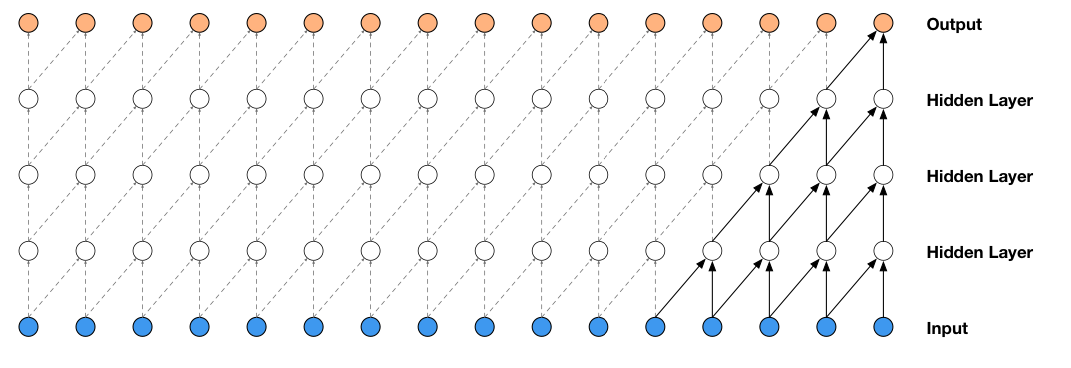
\includegraphics[scale=0.3]{CausalConvolutions.png}
Figure : Visualization of a Stack of causal Convolutional Layers 
\linebreak
Source : [@paper_oord_dieleman_2016]

\end{frame}
%%%%%%%%%%%%%%%%%%%%%%%%%%%%%%%%%%%%%%%%%%%%%%%%%%%%%%%%%%%%%%%%%%%%%%%

## Causal Convolutions

### Model Explanation - Causal Convolutions

- Main Ingredient of WaveNet are Causal Convolutions
- Based on that, the Model cannot violate the Ordering in which the Data is modeled
- Predictions emitted by the Model at Timestep t cannot depend on any of the future Timesteps
- At Training, Conditional Predictions for all Timesteps can be made in parallel ( all Timesteps of Ground Truth x are known )

\vspace{1cm}
Source : [@paper_oord_dieleman_2016]
\end{frame}
%%%%%%%%%%%%%%%%%%%%%%%%%%%%%%%%%%%%%%%%%%%%%%%%%%%%%%%%%%%%%%%%%%%%%%%

### Model Explanation - Causal Convolutions

- At the Generation of the Outputs with the Model, Predictions are sequential : \linebreak
    after each Sample is predicted, it is fed back into the Network to predict the next Sample
- Models with Causal Convolutions do not have recurrent Connections, they are typically faster to train than RNNs
- Problem of Causal Convolutions is : they require many Layers, or large Filters to increase the Receptive Field

\vspace{1cm}
Source : [@paper_oord_dieleman_2016]
\end{frame}
%%%%%%%%%%%%%%%%%%%%%%%%%%%%%%%%%%%%%%%%%%%%%%%%%%%%%%%%%%%%%%%%%%%%%%%

## Dilated Convolutions

### Model Explanation - Dilated Convolutions

- A Dilated Convolution is a Convolution where the Filter is applied over an area larger than its length by skipping Input Values with a certain step
- It is equivalent to a Convolution with a larger Filter derived from the original Filter by dilating it with zeros, but significantly more efficient
- Similar to pooling or strided Convolutions, but here the Output has the same Size as the Input
- Stacked Dilated Convolutions enable Networks to have very large receptive Fields with just a few Layers

\vspace{1cm}
Source : [@paper_oord_dieleman_2016]
\end{frame}
%%%%%%%%%%%%%%%%%%%%%%%%%%%%%%%%%%%%%%%%%%%%%%%%%%%%%%%%%%%%%%%%%%%%%%%

### Model Explanation - Visual

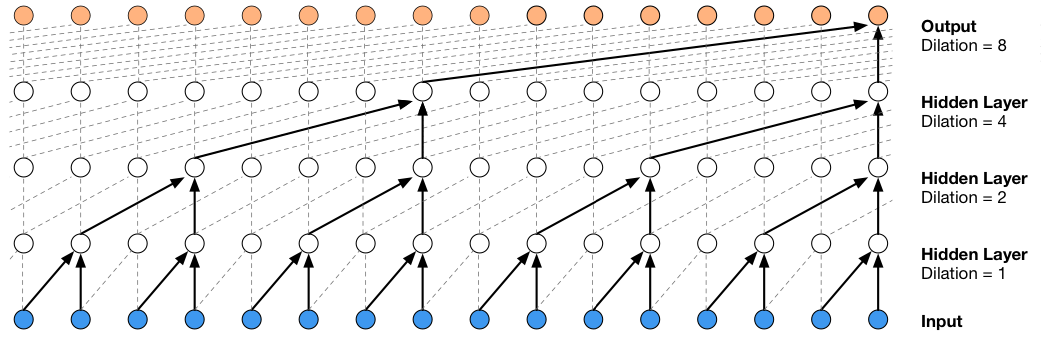
\includegraphics[scale=0.3]{DilatedCausalConvolutions.png}
Figure : Visualization of a stack of Dilated Causal Convolutional Layers
\linebreak
Source: [@paper_oord_dieleman_2016]

\end{frame}
%%%%%%%%%%%%%%%%%%%%%%%%%%%%%%%%%%%%%%%%%%%%%%%%%%%%%%%%%%%%%%%%%%%%%%%

# Music Production with WaveNet

### Music Production with WaveNet

- "WaveNets can be used to model any audio signal"
\linebreak
- Unlike the TTS experiments Networks were not conditioned on an Input Sequence telling it what to play (such as a musical score)
- Instead : simply let it generate whatever it wanted to
- Fact that directly generating Timestep per Timestep with Deep Neural Networks works at all for 16kHz Audio is really surprising

\vspace{1cm}
Source : [@webpage_oord_dieleman_2016]
\end{frame}
%%%%%%%%%%%%%%%%%%%%%%%%%%%%%%%%%%%%%%%%%%%%%%%%%%%%%%%%%%%%%%%%%%%%%%%

# Implementation Example

### Implementation Example

Let's have a look at the Results Chen written down in \linebreak
following Article :

\begin{center}
    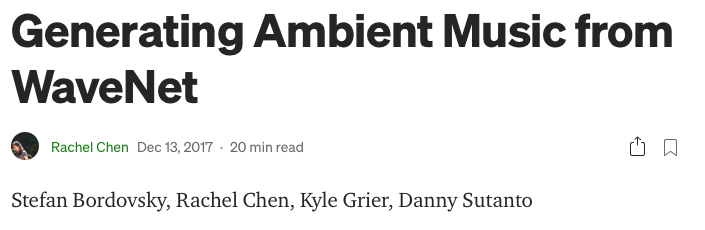
\includegraphics[scale=0.3]{medium.png}
\end{center}

\vspace{1cm}
Source : Medium [@chen_2017]
\end{frame}
%%%%%%%%%%%%%%%%%%%%%%%%%%%%%%%%%%%%%%%%%%%%%%%%%%%%%%%%%%%%%%%%%%%%%%%

## Prerequisites

### Implementation Example - Prerequisites

- The Model trained on Tensorflow Implementation of WaveNet
- 150 000 Steps at a default of 0.001 Learning Rate
- They use Amazon Web Services’ p2.xLarge EC2 Instance to train the WaveNet Model with a GPU
- 118 500 Steps trained in approximately 3.5 days ( then the AWS Costs get to high ) : 
    * With each Step taking roughly 2.5 seconds
    * Their Notebooks took approximately 1 Minute just to train one Step

\vspace{1cm}
Source : Medium [@chen_2017]
\end{frame}
%%%%%%%%%%%%%%%%%%%%%%%%%%%%%%%%%%%%%%%%%%%%%%%%%%%%%%%%%%%%%%%%%%%%%%%

## Results

### Implementation Example - Some Results

- Based on Happy Music from YouTube the Model Results are : \linebreak
    * \href{https://soundcloud.com/rachachachara/happy-9950-generated?utm_source=clipboard&utm_campaign=wtshare&utm_medium=widget&utm_content=https\%253A\%252F\%252Fsoundcloud.com\%252Frachachachara\%252Fhappy-9950-generated}{\beamergotobutton{9950 steps}} \linebreak
    * \href{https://soundcloud.com/rachachachara/happy-10800-generated?utm_source=clipboard&utm_campaign=wtshare&utm_medium=widget&utm_content=https\%253A\%252F\%252Fsoundcloud.com\%252Frachachachara\%252Fhappy-10800-generated}{\beamergotobutton{10800 steps}}\linebreak
    * \href{https://soundcloud.com/rachachachara/happy-14450-generated?utm_source=clipboard&utm_campaign=wtshare&utm_medium=widget&utm_content=https\%253A\%252F\%252Fsoundcloud.com\%252Frachachachara\%252Fhappy-14450-generated}{\beamergotobutton{14450 steps}}\linebreak
    * \href{https://soundcloud.com/rachachachara/happy-25650-long-generated?utm_source=clipboard&utm_campaign=wtshare&utm_medium=widget&utm_content=https\%253A\%252F\%252Fsoundcloud.com\%252Frachachachara\%252Fhappy-25650-long-generated}{\beamergotobutton{25650 steps}}

\vspace{1cm}
Source : Medium [@chen_2017]
\end{frame}
%%%%%%%%%%%%%%%%%%%%%%%%%%%%%%%%%%%%%%%%%%%%%%%%%%%%%%%%%%%%%%%%%%%%%%%

## Challenges

### Implementation Example - Challenges

- Very much Iterations are needed in order to achieve approximately good Results
- The Model requires at least 20 000 Steps to generate something somewhat recognizable
- And around 80 000 Steps for something somewhat coherent
- Learning on local Machines takes very long for only semi good results

\vspace{1cm}
Source : Medium [@chen_2017]
\end{frame}
%%%%%%%%%%%%%%%%%%%%%%%%%%%%%%%%%%%%%%%%%%%%%%%%%%%%%%%%%%%%%%%%%%%%%%%

## Chances

### Implementation Example - Chances

- Scientist at DeepMind implemented a Model playing Piano : 
    * \href{https://storage.googleapis.com/deepmind-media/research/WaveNet/Music/sample_1.wav}{\beamergotobutton{WaveNet Piano example}} [@webpage_oord_dieleman_2016]
- Advantage is, that they input exactly one Instrument
- WaveNet achieves good results on simple Inputs
- Complex Inputs require a lot of Learning Steps

\end{frame}
%%%%%%%%%%%%%%%%%%%%%%%%%%%%%%%%%%%%%%%%%%%%%%%%%%%%%%%%%%%%%%%%%%%%%%%

# Wrap up

### Wrap up

- WaveNet is basically a good Model for generating Music
- Good Results can be achieved quickly with individual Instruments
- If whole songs are used as Input, the Model has to make significantly more Learning Steps
- This extensive learning is very Computationally, Time-Consuming and Costly

\end{frame}
%%%%%%%%%%%%%%%%%%%%%%%%%%%%%%%%%%%%%%%%%%%%%%%%%%%%%%%%%%%%%%%%%%%%%%%



%%novalidate
\end{markdown}

\begin{frame}
\renewcommand{\bibfont}{\footnotesize}
\frametitle{Bibliography}

\bibliographystyle{apalike}
\bibliography{refs}

\end{frame}


\end{document}
